% --- IMPORTS ---
\documentclass[leqno]{article}
\usepackage{graphicx}
\usepackage{dsfont}
\usepackage{mathtools}
\usepackage{amssymb}
\usepackage{amsmath}
\usepackage{amsthm}
\usepackage{float}
\usepackage{ragged2e}
\usepackage{tensor}
\usepackage{fancyhdr}
\usepackage{empheq}
\usepackage[most]{tcolorbox}
\usepackage{enumitem}
\usepackage{dirtytalk}
\usepackage{marginnote}
\usepackage{microtype}
\usepackage[
  a4paper,
  left=0.8in,
  right=1in,
  top=1in,
  bottom=0.5in,
  headheight=14pt,
  headsep=0.4in
]{geometry}
\setlength{\parindent}{0cm}
% --- TikZ Packages ---
\usepackage{pgfplots}
\pgfplotsset{compat=1.18}
\usepgfplotslibrary{fillbetween, polar}
\usetikzlibrary{calc, positioning}
\usetikzlibrary{angles, quotes}
\usetikzlibrary{arrows.meta}
\usetikzlibrary{decorations.pathreplacing, decorations.markings}
\usetikzlibrary{patterns}
\usetikzlibrary{intersections}
% --- URL Packages ---
\usepackage[colorlinks=true,linkcolor=red,citecolor=magenta,urlcolor=black]{hyperref}%
\urlstyle{same}
% --- END OF IMPORTS ---

% --- CUSTOM COMMANDS ---
\RenewDocumentCommand{\marks}{o m}{%
  \IfValueTF{#1}%
    {\marginnote{\raggedright\textbf{[#2]}}[#1]}%
    {\marginnote{\raggedright\textbf{[#2]}}}%
}
\newcommand{\vspacerule}[2]{%
  \par\vspace*{#1}%
  \noindent\hrulefill\par
  \vspace*{#2}%
}
\definecolor{scarlet}{RGB}{205, 40, 75}
\newcommand{\questionitem}{%
  \item\phantomsection
  \addcontentsline{toc}{section}{Question \number\value{enumi}}%
}
\renewcommand{\contentsname}{Questions}
\newcommand{\timingbox}[4]{%
  \vspace*{20pt}
  \noindent\begin{tcolorbox}[
    enhanced, sharp corners,
    width=0.8\textwidth,
    colback=white, colframe=white, boxrule=0pt,
    borderline west={3pt}{0pt}{scarlet},
    left=20pt, right=20pt, top=12pt, bottom=12pt,
    before skip=0pt, after skip=0pt
  ]
  {\LARGE\bfseries #1}\\[8pt]
  {\normalsize Total Marks: #2 }\\[6pt]
  {\normalsize  #3\\[6pt]
  Complete in \textbf{#4}}
  \end{tcolorbox}
  \vspace*{20pt}%
}
% --- END OF CUSTOM COMMANDS ---

% --- HEADER CONFIG ---
\pagestyle{fancy}
\fancyhead{}
\fancyfoot{}
\renewcommand{\headrulewidth}{0.9pt}
\lhead{\textit{Solutions} - Collisions in 2 Dimensions}
\chead{}
\rhead{\href{https://danieljsmith.org}{danieljsmith.org}}
% --- END OF HEADER CONFIG ---

\begin{document}
\vspace*{20pt}
\tableofcontents
\newpage
\begin{enumerate}[
  label=\textbf{\arabic*.},
  leftmargin=*,
  topsep=0pt,
  partopsep=0pt,
  parsep=0pt
]

% ---- Question 1 ----
\questionitem
% [Source: _QBT___Solns__Collisions_in_2_Dimensions, Q1]

\begin{figure}[H]
    \centering
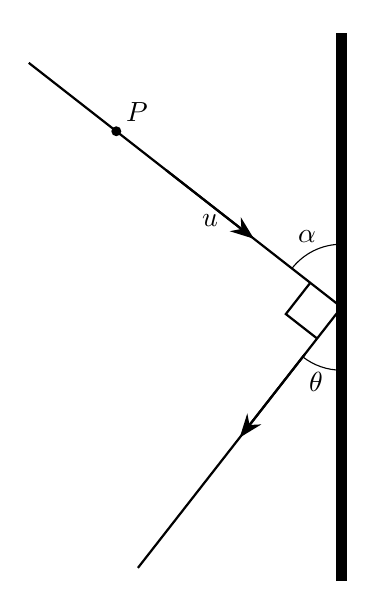
\begin{tikzpicture}[scale=1.2]
\def\alphaang{52}
\def\thetaang{38}
\def\inclen{4.2}
\def\outlen{3.5}
\def\wallht{2.9}
\def\marklen{0.42}

\coordinate (C) at (0,0);
\coordinate (U) at (0,1.5);
\coordinate (D) at (0,-1.5);
\coordinate (I) at ({90+\alphaang}:\inclen);
\coordinate (R) at ({270-\thetaang}:\outlen);
\coordinate (P) at ($(C)!0.72!(I)$);
\coordinate (uA) at ($(C)!0.28!(I)$);
\coordinate (uB) at ($(C)!0.56!(I)$);
\coordinate (vA) at ($(C)!0.18!(R)$);
\coordinate (vB) at ($(C)!0.50!(R)$);
\coordinate (Q1) at ({90+\alphaang}:\marklen);
\coordinate (Q2) at ({270-\thetaang}:\marklen);
\coordinate (Q3) at ($(Q1)+(Q2)-(C)$);

\draw[line width=4pt] (0,-\wallht) -- (0,\wallht);
\draw[thick] (I) -- (C) -- (R);

\draw[-{Stealth[length=3mm]}, thick] (uB) -- (uA) node[midway, below] {$u$};
\draw[-{Stealth[length=3mm]}, thick] (vA) -- (vB);

\draw[thick] (Q1) -- (Q3) -- (Q2);

\fill (P) circle (1.5pt);
\node[above right] at (P) {$P$};

\pic["$\alpha$", draw, angle radius=8mm, angle eccentricity=1.25] {angle=U--C--I};
\pic["$\theta$", draw, angle radius=8mm, angle eccentricity=1.25] {angle=R--C--D};
\end{tikzpicture}
\end{figure}


A particle $P$ of mass $m$ is moving with speed $u$ on a fixed smooth horizontal surface. It collides with a fixed smooth vertical barrier. Before impact its path makes an angle $\alpha$ with the barrier, and after impact its path makes an angle $\theta$ with the barrier. The incident path and the outgoing path are perpendicular. The coefficient of restitution between $P$ and the barrier is $e$. The particle loses $36\%$ of its kinetic energy in the collision. \\

Find the value of $e$ and the exact value of $\tan \alpha$. \marks{5}

\vspace*{10pt}

\begin{tcolorbox}[colback=white, colframe=scarlet, title={\textbf{Solution}}, breakable, grow to left by=6mm, grow to right by=10mm]
Take components parallel and perpendicular to the barrier.

Before impact:
\[
\text{parallel component}=u\cos\alpha,\qquad \text{perpendicular component}=u\sin\alpha
\]

Since the barrier is smooth, the component parallel to the barrier is unchanged, and the perpendicular component is reversed in direction and multiplied by \(e\). So after impact:
\[
\text{parallel component}=u\cos\alpha,\qquad \text{perpendicular component}=eu\sin\alpha
\]

Because the incident path and outgoing path are perpendicular, and both angles are measured from the barrier,
\[
\alpha+\theta=90^\circ
\]
Hence
\[
\tan\theta=\cot\alpha=\frac{1}{\tan\alpha}
\]

But from the components after impact,
\[
\tan\theta=\frac{eu\sin\alpha}{u\cos\alpha}=e\tan\alpha
\]

So
\[
e\tan\alpha=\frac{1}{\tan\alpha}
\]
which gives
\[
e\tan^2\alpha=1
\]

Now use the kinetic energy information.

The particle loses \(36\%\) of its kinetic energy, so it keeps \(64\%\) of it.

Initial kinetic energy:
\[
\frac12 mu^2
\]

After impact, the speed is
\[
\sqrt{(u\cos\alpha)^2+(eu\sin\alpha)^2}
\]
so the kinetic energy after impact is
\[
\frac12 m\left((u\cos\alpha)^2+(eu\sin\alpha)^2\right)
=\frac12 mu^2\left(\cos^2\alpha+e^2\sin^2\alpha\right)
\]

Therefore
\[
\frac12 mu^2\left(\cos^2\alpha+e^2\sin^2\alpha\right)
=\frac{64}{100}\cdot \frac12 mu^2
\]
so
\[
\cos^2\alpha+e^2\sin^2\alpha=\frac{16}{25}
\]

From
\[
e\tan^2\alpha=1
\]
we have
\[
e\frac{\sin^2\alpha}{\cos^2\alpha}=1
\]
hence
\[
e\sin^2\alpha=\cos^2\alpha
\]

Using this in the energy equation,
\begin{align*}
\cos^2\alpha+e^2\sin^2\alpha
&=e\sin^2\alpha+e^2\sin^2\alpha \\
&=e(1+e)\sin^2\alpha
\end{align*}

Also, since \(\cos^2\alpha+\sin^2\alpha=1\),
\[
e\sin^2\alpha+\sin^2\alpha=(1+e)\sin^2\alpha=1
\]
So
\[
e(1+e)\sin^2\alpha=e
\]

Therefore
\[
\cos^2\alpha+e^2\sin^2\alpha=e
\]
and hence
\[
e=\frac{16}{25}
\]

Finally,
\[
\tan^2\alpha=\frac{1}{e}=\frac{25}{16}
\]
Since \(\alpha\) is acute,
\[
\tan\alpha=\frac54
\]

So the required values are
\[
e=\frac{16}{25},\qquad \tan\alpha=\frac54
\]
\end{tcolorbox}


\newpage

% ---- Question 2 ----
\questionitem
% [Source: _QBT___Solns__Collisions_in_2_Dimensions, Q2]

A hockey puck moving on a smooth horizontal rink collides with a fixed straight side-board. \\
Let $\mathbf{i}$ be a unit vector parallel to the side-board and let $\mathbf{j}$ be a unit vector perpendicular to the side-board, directed away from it. \\

Immediately before the collision, the puck has velocity $(9\mathbf{i}-12\mathbf{j})\,\mathrm{m\,s^{-1}}$. \\

Immediately after the collision, the puck moves with speed $10\,\mathrm{m\,s^{-1}}$ in the direction of the vector $3\mathbf{i}+4\mathbf{j}$. \\

Model the puck as a particle. \\

\begin{enumerate}[label=\textbf{(\alph*)}]
  \item Find the coefficient of restitution between the puck and the side-board. \marks{3} \\
  \item Determine whether or not the side-board is smooth.

  Fully justify your answer. \marks{3} \\
\end{enumerate}

\vspace*{10pt}

\begin{tcolorbox}[colback=white, colframe=scarlet, title={\textbf{Solution}}, breakable, grow to left by=6mm, grow to right by=10mm]
\begin{enumerate}[label=\textbf{(\alph*)}]
  \item The direction after collision is along $3\mathbf{i}+4\mathbf{j}$, whose magnitude is
\[
\sqrt{3^2+4^2}=5
\]
So the velocity immediately after collision is
\[
10\times \frac{3\mathbf{i}+4\mathbf{j}}{5}=6\mathbf{i}+8\mathbf{j}
\]

For a collision with a fixed side-board, the coefficient of restitution is
\[
e=\frac{\text{speed of separation perpendicular to board}}{\text{speed of approach perpendicular to board}}
\]

Before collision, the perpendicular component is $-12\mathbf{j}$, so the speed of approach is $12$.

After collision, the perpendicular component is $8\mathbf{j}$, so the speed of separation is $8$.

Hence
\[
e=\frac{8}{12}=\frac{2}{3}
\]

So the coefficient of restitution is $\dfrac{2}{3}$.

  \item The component of velocity parallel to the side-board is the $\mathbf{i}$-component.

Before collision, this is
\[
9\text{ m s}^{-1}
\]

After collision, from part (a), the velocity is $6\mathbf{i}+8\mathbf{j}$, so the parallel component is
\[
6\text{ m s}^{-1}
\]

If the side-board were smooth, there would be no impulse parallel to the board, so the parallel component of velocity would be unchanged.

But here it changes from $9$ to $6$.

Therefore the side-board is not smooth.
\end{enumerate}
\end{tcolorbox}


\newpage

% ---- Question 3 ----
\questionitem
% [Source: _QBT___Solns__Collisions_in_2_Dimensions, Q3]

\begin{figure}[H]
    \centering
\begin{tikzpicture}[scale=1.2]
\def\w{5.4}
\def\h{4.8}
\def\xD{2.05}
\def\yE{2.6}
\tikzset{traj/.style={thick, postaction={decorate}, decoration={markings, mark=at position 0.55 with {\arrow{Stealth[length=3mm]}}}}}

\coordinate (A) at (0,0);
\coordinate (B) at (\w,0);
\coordinate (C) at (\w,\h);
\coordinate (D) at (\xD,0);
\coordinate (E) at (\w,\yE);
\coordinate (P) at ($(D)+(-3.2,2.0)$);
\coordinate (F) at ($(E)+(-2.8,1.7)$);

\draw[thick] (A) -- (B) -- (C);
\draw[traj] (P) -- (D) node[pos=0.45, above] {$u$};
\draw[traj] (D) -- (E);
\draw[traj] (E) -- (F);

\draw ($(B)+(-0.24,0)$) -- ($(B)+(-0.24,0.24)$) -- ($(B)+(0,0.24)$);

\pic["$\alpha$", draw, angle radius=6mm, angle eccentricity=1.35] {angle=P--D--A};
\pic["$\beta$", draw, angle radius=5mm, angle eccentricity=1.55] {angle=D--E--B};
\pic["$\gamma$", draw, angle radius=5mm, angle eccentricity=1.4] {angle=C--E--F};

\fill (P) circle (1.2pt);
\node[above] at (A) {$A$};
\node[below right] at (B) {$B$};
\node[above right] at (C) {$C$};
\node[above left] at (P) {$P$};
\end{tikzpicture}
\end{figure}


The smooth walls $AB$ and $BC$ are at right angles to each other. A particle $P$ moves on a smooth horizontal floor with speed $u$ and strikes the wall $AB$ at an angle $\alpha$ to $AB$. It rebounds, then strikes the wall $BC$ at an angle $\beta$ to $BC$. After the second impact it rebounds at an angle $\gamma$ to $BC$, as shown in the diagram. The coefficient of restitution between $P$ and each wall is $e$. \\

\begin{enumerate}[label=\textbf{(\alph*)}]
  \item Show that
  \[
  \tan \alpha \tan \beta = \dfrac{1}{e}
  \] \marks[-20pt]{3}
  \item Express $\gamma$ in terms of $\alpha$ and explain what this implies about the final direction of motion of $P$. \marks{4} \\
\end{enumerate}
During the first impact the particle loses four times as much kinetic energy as it loses during the second impact. After the second impact the kinetic energy of $P$ is $\dfrac{9}{25}$ of its initial kinetic energy. \\

\begin{enumerate}[label=\textbf{(\alph*)}, resume]
  \item Find the value of $e$ and the value of $\tan \alpha$. \marks{4} \\
\end{enumerate}

\vspace*{10pt}

\begin{tcolorbox}[colback=white, colframe=scarlet, title={\textbf{Solution}}, breakable, grow to left by=6mm, grow to right by=10mm]
\begin{enumerate}[label=\textbf{(\alph*)}]
  \item Take $AB$ to be horizontal and $BC$ vertical.

  Before the first impact, since the particle strikes $AB$ at angle $\alpha$ to the wall,
  \[
  \text{component parallel to }AB=u\cos\alpha,\qquad
  \text{component perpendicular to }AB=u\sin\alpha
  \]

  For impact with a smooth wall, the component parallel to the wall is unchanged, and the component perpendicular to the wall is reversed and multiplied by $e$.

  So after rebounding from $AB$,
  \[
  \text{horizontal component}=u\cos\alpha,\qquad
  \text{vertical component}=eu\sin\alpha
  \]

  At $BC$, the angle $\beta$ is measured with the wall $BC$, so
  \[
  \tan\beta=\frac{\text{component perpendicular to }BC}{\text{component parallel to }BC}
  =\frac{u\cos\alpha}{eu\sin\alpha}
  =\frac{1}{e\tan\alpha}
  \]

  Hence
  \[
  \tan\alpha\tan\beta=\frac{1}{e}
  \]

  \item Just before the second impact with $BC$, the velocity components are
  \[
  (u\cos\alpha,\ eu\sin\alpha)
  \]

  On rebounding from the smooth wall $BC$:
  \begin{itemize}
    \item the component parallel to $BC$ is unchanged,
    \item the component perpendicular to $BC$ is reversed and multiplied by $e$.
  \end{itemize}

  So after the second impact, the velocity components are
  \[
  (-eu\cos\alpha,\ eu\sin\alpha)
  \]

  Therefore
  \[
  \tan\gamma=\frac{\text{component perpendicular to }BC}{\text{component parallel to }BC}
  =\frac{eu\cos\alpha}{eu\sin\alpha}
  =\cot\alpha
  \]

  Hence
  \[
  \tan\gamma=\tan\left(\frac{\pi}{2}-\alpha\right)
  \]

  Since $\gamma$ is an acute angle,
  \[
  \gamma=\frac{\pi}{2}-\alpha
  \]

  Also, the initial velocity was
  \[
  (u\cos\alpha,\ -u\sin\alpha)
  \]
  and the final velocity is
  \[
  (-eu\cos\alpha,\ eu\sin\alpha)=-e(u\cos\alpha,\ -u\sin\alpha)
  \]

  So the final velocity is a negative multiple of the initial velocity. Therefore the final direction of motion is parallel to the initial direction, but in the opposite sense.

  \item After the second impact, the speed is
  \[
  \sqrt{(eu\cos\alpha)^2+(eu\sin\alpha)^2}=eu
  \]

  So
  \[
  \frac{\text{final KE}}{\text{initial KE}}
  =\frac{\frac12 m(eu)^2}{\frac12 mu^2}
  =e^2
  \]

  Given that the final kinetic energy is $\dfrac{9}{25}$ of the initial kinetic energy,
  \[
  e^2=\frac{9}{25}
  \]
  and since $0<e<1$,
  \[
  e=\frac35
  \]

  Now find the losses in kinetic energy.

  Before the first impact, KE $=\dfrac12 mu^2$.

  After the first impact, speed squared is
  \[
  (u\cos\alpha)^2+(eu\sin\alpha)^2
  \]
  so the loss in the first impact is
  \begin{align*}
  \Delta E_1
  &=\frac12 mu^2-\frac12 m\left((u\cos\alpha)^2+(eu\sin\alpha)^2\right) \\
  &=\frac12 mu^2\left(1-\cos^2\alpha-e^2\sin^2\alpha\right) \\
  &=\frac12 mu^2(1-e^2)\sin^2\alpha
  \end{align*}

  Just before the second impact, KE is
  \[
  \frac12 m\left((u\cos\alpha)^2+(eu\sin\alpha)^2\right)
  \]
  and just after the second impact, KE is
  \[
  \frac12 m\left((eu\cos\alpha)^2+(eu\sin\alpha)^2\right)
  \]
  so the loss in the second impact is
  \begin{align*}
  \Delta E_2
  &=\frac12 m\left((u\cos\alpha)^2+(eu\sin\alpha)^2-(eu\cos\alpha)^2-(eu\sin\alpha)^2\right) \\
  &=\frac12 mu^2\left(\cos^2\alpha-e^2\cos^2\alpha\right) \\
  &=\frac12 mu^2(1-e^2)\cos^2\alpha
  \end{align*}

  Given that the first loss is four times the second loss,
  \[
  \Delta E_1=4\Delta E_2
  \]
  so
  \[
  \frac12 mu^2(1-e^2)\sin^2\alpha
  =4\left(\frac12 mu^2(1-e^2)\cos^2\alpha\right)
  \]

  Cancelling the common factor $\dfrac12 mu^2(1-e^2)$ gives
  \[
  \sin^2\alpha=4\cos^2\alpha
  \]
  hence
  \[
  \tan^2\alpha=4
  \]

  Since $\alpha$ is acute,
  \[
  \tan\alpha=2
  \]

  Therefore
  \[
  e=\frac35,\qquad \tan\alpha=2
  \]
\end{enumerate}
\end{tcolorbox}


\newpage

% ---- Question 4 ----
\questionitem
% [Source: _QBT___Solns__Collisions_in_2_Dimensions, Q4]

\begin{figure}[H]
    \centering
\begin{tikzpicture}[scale=1.1]
\def\wallx{4}
\def\wally{-3}
\def\wls{1.0}
\def\wrs{1.2}
\def\uvx{13}
\def\uvy{9}
\def\uis{0.28}
\def\vvx{-2}
\def\vvy{-11}
\def\vos{0.28}

\coordinate (P) at (0,0);
\coordinate (A) at ({-\wls*\wallx},{-\wls*\wally});
\coordinate (B) at ({\wrs*\wallx},{\wrs*\wally});
\coordinate (VinStart) at ({-\uis*\uvx},{-\uis*\uvy});
\coordinate (VoutEnd) at ({\vos*\vvx},{\vos*\vvy});

\draw[thick] (A) -- (B);
\node[above left] at (A) {$A$};
\node[below right] at (B) {$B$};

\draw[-{Stealth[length=3mm]}, thick] (VinStart) -- (P)
    node[pos=0.55, above left] {$(13\mathbf{i}+9\mathbf{j})\,\mathrm{m\,s^{-1}}$};
\draw[-{Stealth[length=3mm]}, thick] (P) -- (VoutEnd)
    node[pos=0.62, below right] {$(-2\mathbf{i}-11\mathbf{j})\,\mathrm{m\,s^{-1}}$};
\end{tikzpicture}
\end{figure}


The diagram above shows the plan view of part of a smooth horizontal table. The line segment $AB$ represents a fixed smooth vertical wall. \\

A small ball of mass $0.4\,\mathrm{kg}$ moves across the table and rebounds after striking the wall. \\

Immediately before impact its velocity is $(13\mathbf{i}+9\mathbf{j})\,\mathrm{m\,s^{-1}}$. \\

Immediately after impact its velocity is $(-2\mathbf{i}-11\mathbf{j})\,\mathrm{m\,s^{-1}}$. \\

The coefficient of restitution between the ball and the wall is $e$. \\

\begin{enumerate}[label=\textbf{(\alph*)}]
  \item Show that $AB$ is parallel to $(4\mathbf{i}-3\mathbf{j})$. \marks{4} \\
  \item Find the value of $e$. \marks{5} \\
\end{enumerate}

\vspace*{10pt}

\begin{tcolorbox}[colback=white, colframe=scarlet, title={\textbf{Solution}}, breakable, grow to left by=6mm, grow to right by=10mm]
\begin{enumerate}[label=\textbf{(\alph*)}]
  \item Let the velocity before impact be
  \[
  \mathbf{u}=13\mathbf{i}+9\mathbf{j}
  \]
  and the velocity after impact be
  \[
  \mathbf{v}=-2\mathbf{i}-11\mathbf{j}
  \]

  The change in velocity is
  \begin{align*}
  \mathbf{v}-\mathbf{u}
  &=(-2-13)\mathbf{i}+(-11-9)\mathbf{j} \\
  &=-15\mathbf{i}-20\mathbf{j} \\
  &=-5(3\mathbf{i}+4\mathbf{j})
  \end{align*}

  When a ball strikes a \emph{smooth} wall, the impulse acts perpendicular to the wall, so the change in velocity is also perpendicular to the wall.

  Hence the wall $AB$ is perpendicular to
  \[
  3\mathbf{i}+4\mathbf{j}
  \]

  A vector perpendicular to $3\mathbf{i}+4\mathbf{j}$ is $4\mathbf{i}-3\mathbf{j}$, since
  \[
  (3\mathbf{i}+4\mathbf{j})\cdot(4\mathbf{i}-3\mathbf{j})=12-12=0
  \]

  Therefore
  \[
  AB \parallel (4\mathbf{i}-3\mathbf{j})
  \]

  \item From part (a), a direction parallel to the wall is $4\mathbf{i}-3\mathbf{j}$, so a direction perpendicular to the wall is $3\mathbf{i}+4\mathbf{j}$.

  Take unit vectors
  \[
  \hat{\mathbf{t}}=\frac{1}{5}(4\mathbf{i}-3\mathbf{j}),
  \qquad
  \hat{\mathbf{n}}=\frac{1}{5}(3\mathbf{i}+4\mathbf{j})
  \]
  where $\hat{\mathbf{t}}$ is parallel to the wall and $\hat{\mathbf{n}}$ is perpendicular to the wall.

  For the velocity before impact,
  \begin{align*}
  \mathbf{u}\cdot\hat{\mathbf{t}}
  &= (13\mathbf{i}+9\mathbf{j})\cdot \frac{1}{5}(4\mathbf{i}-3\mathbf{j}) \\
  &= \frac{1}{5}(52-27) \\
  &= 5
  \end{align*}
  \begin{align*}
  \mathbf{u}\cdot\hat{\mathbf{n}}
  &= (13\mathbf{i}+9\mathbf{j})\cdot \frac{1}{5}(3\mathbf{i}+4\mathbf{j}) \\
  &= \frac{1}{5}(39+36) \\
  &= 15
  \end{align*}

  So before impact, the component parallel to the wall is $5$, and the component perpendicular to the wall is $15$ towards the wall.

  For the velocity after impact,
  \begin{align*}
  \mathbf{v}\cdot\hat{\mathbf{t}}
  &= (-2\mathbf{i}-11\mathbf{j})\cdot \frac{1}{5}(4\mathbf{i}-3\mathbf{j}) \\
  &= \frac{1}{5}(-8+33) \\
  &= 5
  \end{align*}
  \begin{align*}
  \mathbf{v}\cdot\hat{\mathbf{n}}
  &= (-2\mathbf{i}-11\mathbf{j})\cdot \frac{1}{5}(3\mathbf{i}+4\mathbf{j}) \\
  &= \frac{1}{5}(-6-44) \\
  &= -10
  \end{align*}

  So after impact, the component parallel to the wall is still $5$, and the perpendicular component has reversed direction with speed $10$ away from the wall.

  Since the wall is fixed,
  \[
  e=\frac{\text{speed of separation}}{\text{speed of approach}}
  \]
  measured perpendicular to the wall. Therefore
  \[
  e=\frac{10}{15}=\frac{2}{3}
  \]

  Hence
  \[
  e=\frac{2}{3}
  \]
\end{enumerate}
\end{tcolorbox}


\newpage

% ---- Question 5 ----
\questionitem
% [Source: _QBT___Solns__Collisions_in_2_Dimensions, Q5]

\begin{figure}[H]
    \centering
\begin{tikzpicture}[scale=1.75]
\def\W{7}
\def\H{3}
\def\ballrad{0.09}
\def\angw{45}
\def\angr{36}
\pgfmathsetmacro{\wx}{1.25}
\pgfmathsetmacro{\wy}{2.05}
\pgfmathsetmacro{\rx}{1.37}
\pgfmathsetmacro{\ry}{1.95}
\pgfmathsetmacro{\xU}{\wx + (\H-\wy)/tan(\angw)}
\pgfmathsetmacro{\xV}{\rx + \ry/tan(\angr)}

\coordinate (A) at (0,\H);
\coordinate (B) at (\W,\H);
\coordinate (C) at (\W,0);
\coordinate (D) at (0,0);
\coordinate (Wc) at (\wx,\wy);
\coordinate (Rc) at (\rx,\ry);
\coordinate (U) at (\xU,\H);
\coordinate (V) at (\xV,0);
\coordinate (Wtip) at ($(Wc)!0.62!(U)$);
\coordinate (Rtip) at ($(Rc)!0.62!(V)$);

\draw[thick] (A) -- (B) -- (C) -- (D) -- cycle;

\draw[thick] (Wc) circle (\ballrad);
\draw[thick] (Rc) circle (\ballrad);

\draw[-{Stealth[length=3mm]}, thick] (Wc) -- (Wtip)
  node[pos=0.54, below right, yshift=4pt] {$\left(\sqrt{3}-1\right)\ \mathrm{m\,s^{-1}}$};
\draw[dashed, thick] (Wtip) -- (U);

\draw[-{Stealth[length=3mm]}, thick] (Rc) -- (Rtip)
  node[pos=0.52, below left] {$v\ \mathrm{m\,s^{-1}}$};
\draw[dashed, thick] (Rtip) -- (V);

\pic["$45^\circ$", draw, angle radius=6mm, angle eccentricity=1.55] {angle=A--U--Wtip};
\pic["$\theta$", draw, angle radius=6mm, angle eccentricity=1.35] {angle=Rtip--V--D};

\node[above left] at (A) {$A$};
\node[above right] at (B) {$B$};
\node[below right] at (C) {$C$};
\node[below left] at (D) {$D$};
\end{tikzpicture}
\end{figure}


Two snooker balls, one white and one red, have equal mass.

The balls are on a horizontal table $ABCD$. \\

The white ball is struck so that it moves at a speed of $2\,\mathrm{m\,s^{-1}}$ in a direction making an angle of $15^\circ$ with $AB$, towards $CD$. \\

The white ball hits a stationary red ball. \\

After the collision, the white ball moves at a speed of $(\sqrt{3}-1)\,\mathrm{m\,s^{-1}}$ and at an angle of $45^\circ$ to $AB$. \\

After the collision, the red ball moves at a speed $v\,\mathrm{m\,s^{-1}}$ and at an angle $\theta$ to $CD$. \\

When the collision takes place, the point of impact is twice as far from $CD$ as it is from $AB$. \\

The diagram below shows the velocities of the balls after the collision. \\

After the collision, the white ball hits $AB$ and the red ball hits $CD$. \\

Model the balls as particles and neglect any resistance. \\

\begin{enumerate}[label=\textbf{(\alph*)}]
  \item Explain why the two balls hit the sides of the table at the same time. \marks{2} \\
  \item Show that $\theta = 36.2^\circ$ correct to one decimal place. \marks{4} \\
  \item Find $v$. \marks{2} \\
  \item Determine which ball travels the greater distance after the collision and before hitting the side of the table.

  Fully justify your answer. \marks{2} \\
  \item State one possible refinement to the model that you have used. \marks{1} \\
\end{enumerate}

\vspace*{10pt}

\begin{tcolorbox}[colback=white, colframe=scarlet, title={\textbf{Solution}}, breakable, grow to left by=6mm, grow to right by=10mm]
\begin{enumerate}[label=\textbf{(\alph*)}]
  \item Let the perpendicular distance from the point of impact to $AB$ be $d$.  
  Then the perpendicular distance to $CD$ is $2d$.

  Since $AB \parallel CD$, the times to reach the sides depend on the velocity components perpendicular to these sides.

  Take perpendicular to $AB$ as positive towards $CD$. Since the masses are equal, conservation of momentum perpendicular to $AB$ gives
  \[
  2\sin 15^\circ = v\sin\theta - (\sqrt3-1)\sin45^\circ
  \]
  so
  \[
  v\sin\theta = 2\sin15^\circ + (\sqrt3-1)\sin45^\circ
  \]

  Now
  \begin{align*}
  2\sin15^\circ &= 2\cdot \frac{\sqrt6-\sqrt2}{4}
  = \frac{\sqrt6-\sqrt2}{2} \\
  (\sqrt3-1)\sin45^\circ &= (\sqrt3-1)\cdot \frac{\sqrt2}{2}
  = \frac{\sqrt6-\sqrt2}{2}
  \end{align*}

  Hence
  \[
  v\sin\theta = \sqrt6-\sqrt2
  \]

  So the red ball moves towards $CD$ with speed component $\sqrt6-\sqrt2$, while the white ball moves towards $AB$ with speed component
  \[
  (\sqrt3-1)\sin45^\circ = \frac{\sqrt6-\sqrt2}{2}
  \]

  Therefore the red ball's perpendicular speed is twice the white ball's, and its perpendicular distance to travel is also twice as great.

  \[
  t_{\text{white}}=\frac{d}{(\sqrt6-\sqrt2)/2},
  \qquad
  t_{\text{red}}=\frac{2d}{\sqrt6-\sqrt2}
  \]

  These are equal, so the two balls hit the sides of the table at the same time.

  \item Since $AB \parallel CD$, the red ball makes the same angle $\theta$ with $AB$ as with $CD$.

  Resolving parallel to $AB$ and using conservation of momentum:
  \[
  2\cos15^\circ = (\sqrt3-1)\cos45^\circ + v\cos\theta
  \]

  Hence
  \begin{align*}
  v\cos\theta
  &= 2\cos15^\circ - (\sqrt3-1)\cos45^\circ \\
  &= 2\cdot \frac{\sqrt6+\sqrt2}{4} - (\sqrt3-1)\cdot \frac{\sqrt2}{2} \\
  &= \frac{\sqrt6+\sqrt2}{2} - \frac{\sqrt6-\sqrt2}{2} \\
  &= \sqrt2
  \end{align*}

  From part (a),
  \[
  v\sin\theta = \sqrt6-\sqrt2
  \]

  Therefore
  \begin{align*}
  \tan\theta
  &= \frac{v\sin\theta}{v\cos\theta}
  = \frac{\sqrt6-\sqrt2}{\sqrt2} \\
  &= \sqrt3-1
  \end{align*}

  So
  \[
  \theta=\tan^{-1}(\sqrt3-1)=36.2^\circ \text{ (to 1 d.p.)}
  \]

  Hence $\theta=36.2^\circ$ correct to one decimal place.

  \item Using the results from part (b),
  \[
  v\cos\theta=\sqrt2,
  \qquad
  v\sin\theta=\sqrt6-\sqrt2
  \]

  So
  \begin{align*}
  v^2
  &= (v\cos\theta)^2 + (v\sin\theta)^2 \\
  &= (\sqrt2)^2 + (\sqrt6-\sqrt2)^2 \\
  &= 2 + (6+2-2\sqrt{12}) \\
  &= 2 + 8 - 4\sqrt3 \\
  &= 10-4\sqrt3
  \end{align*}

  Hence
  \[
  v=\sqrt{10-4\sqrt3}\ \mathrm{m\,s^{-1}}
  \]

  Since speed is positive,
  \[
  v=\sqrt{10-4\sqrt3}\ \mathrm{m\,s^{-1}} \approx 1.75\ \mathrm{m\,s^{-1}}
  \]

  \item From part (a), both balls travel for the same time after the collision.

  Let this common time be $t$. Then the distances travelled are
  \[
  s_{\text{white}}=(\sqrt3-1)t,
  \qquad
  s_{\text{red}}=vt
  \]

  From part (c),
  \[
  v=\sqrt{10-4\sqrt3}\approx 1.75
  \]
  and
  \[
  \sqrt3-1\approx 0.732
  \]

  Since
  \[
  1.75 > 0.732
  \]
  we have
  \[
  s_{\text{red}} > s_{\text{white}}
  \]

  Therefore the red ball travels the greater distance after the collision and before hitting the side of the table.

  \item One possible refinement is to include friction (or rolling resistance) between the balls and the table.
\end{enumerate}
\end{tcolorbox}


\newpage

% ---- Question 6 ----
\questionitem
% [Source: _QBT___Solns__Collisions_in_2_Dimensions, Q6]

\begin{figure}[H]
    \centering
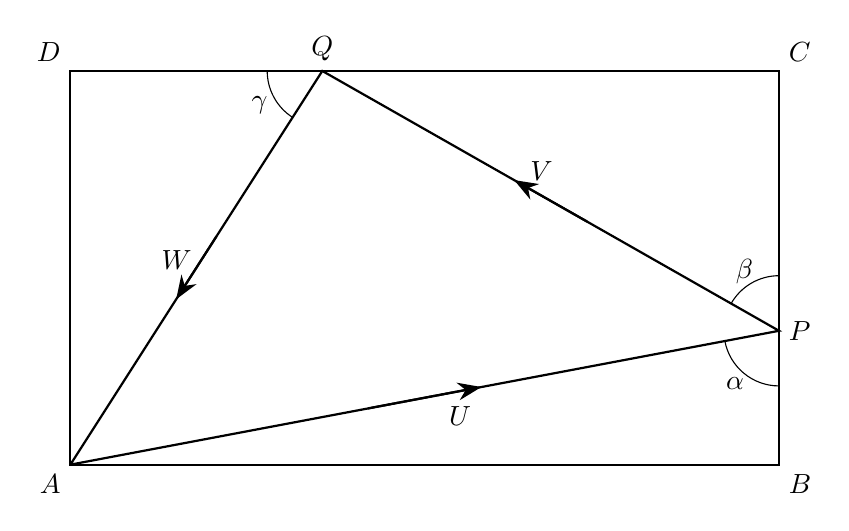
\begin{tikzpicture}[scale=1.0]
\def\W{9}
\def\H{5}
\def\Py{1.7}
\def\Qx{3.2}

\coordinate (A) at (0,0);
\coordinate (B) at (\W,0);
\coordinate (C) at (\W,\H);
\coordinate (D) at (0,\H);
\coordinate (P) at (\W,\Py);
\coordinate (Q) at (\Qx,\H);

\draw[thick] (A) -- (B) -- (C) -- (D) -- cycle;
\draw[thick] (A) -- (P) -- (Q) -- (A);

\draw[-{Stealth[length=3mm]}, thick] ($(A)!0.42!(P)$) -- ($(A)!0.58!(P)$);
\draw[-{Stealth[length=3mm]}, thick] ($(P)!0.42!(Q)$) -- ($(P)!0.58!(Q)$);
\draw[-{Stealth[length=3mm]}, thick] ($(Q)!0.42!(A)$) -- ($(Q)!0.58!(A)$);

\node[below, yshift=-2pt] at ($(A)!0.55!(P)$) {$U$};
\node[above, yshift=2pt] at ($(P)!0.52!(Q)$) {$V$};
\node[left] at ($(Q)!0.48!(A)$) {$W$};

\pic["$\alpha$", draw, angle radius=7mm, angle eccentricity=1.25] {angle=A--P--B};
\pic["$\beta$", draw, angle radius=7mm, angle eccentricity=1.25] {angle=C--P--Q};
\pic["$\gamma$", draw, angle radius=7mm, angle eccentricity=1.3] {angle=D--Q--A};

\node[below left] at (A) {$A$};
\node[below right] at (B) {$B$};
\node[above right] at (C) {$C$};
\node[above left] at (D) {$D$};
\node[right] at (P) {$P$};
\node[above] at (Q) {$Q$};
\end{tikzpicture}
\end{figure}


A small smooth billiard ball is projected from the corner $A$ of a horizontal rectangular table $ABCD$. \\

The ball first hits the side $BC$ at the point $P$, then hits the side $CD$ at the point $Q$, and then returns to $A$. \\

Angle $APB=\alpha$, angle $CPQ=\beta$ and angle $DQA=\gamma$. \\

The ball moves along $AP$ with speed $U$, along $PQ$ with speed $V$ and along $QA$ with speed $W$, as shown in the diagram. \\

The coefficient of restitution between the ball and side $BC$ is $e_1$. \\

The coefficient of restitution between the ball and side $CD$ is $e_2$. \\

The ball is modelled as a particle. \\

\begin{enumerate}[label=\textbf{(\alph*)}]
  \item Show that $\tan\beta=e_1\tan\alpha$. \marks{4} \\
  \item Hence show that $e_1\tan\alpha\tan\gamma=e_2$. \marks{3} \\
  \item By considering $\angle PAQ$ or otherwise, show that it is possible for the ball to return to $A$ only if $e_2>e_1$. \marks{6} \\
\end{enumerate}

If instead $e_1=e_2$, the ball would not return to $A$. \\

\begin{enumerate}[label=\textbf{(\alph*)}, resume]
  \item Given that $e_1=e_2$, use the result from part (b) to describe the path of the ball after it hits $CD$ at $Q$, explaining your answer. \marks{1} \\
\end{enumerate}

\vspace*{10pt}

\begin{tcolorbox}[colback=white, colframe=scarlet, title={\textbf{Solution}}, breakable, grow to left by=6mm, grow to right by=10mm]
\begin{enumerate}[label=\textbf{(\alph*)}]
  \item At the first impact, the ball hits the side $BC$.

  For a smooth side:
  \begin{itemize}
    \item the component of velocity \emph{parallel} to the side is unchanged,
    \item the component of velocity \emph{perpendicular} to the side is reversed and multiplied by the coefficient of restitution.
  \end{itemize}

  Resolve the velocity relative to $BC$.

  Before impact, along $AP$ with speed $U$:
  \[
  \text{parallel to }BC = U\cos\alpha, 
  \qquad
  \text{perpendicular to }BC = U\sin\alpha
  \]

  After impact, along $PQ$ with speed $V$:
  \[
  \text{parallel to }BC = V\cos\beta, 
  \qquad
  \text{perpendicular to }BC = V\sin\beta
  \]

  So
  \begin{align*}
  V\cos\beta &= U\cos\alpha \\
  V\sin\beta &= e_1U\sin\alpha
  \end{align*}

  Dividing the second equation by the first,
  \begin{align*}
  \frac{V\sin\beta}{V\cos\beta}
  &= \frac{e_1U\sin\alpha}{U\cos\alpha} \\
  \tan\beta &= e_1\tan\alpha
  \end{align*}

  Hence
  \[
  \tan\beta = e_1\tan\alpha
  \]

  \item At the second impact, the ball hits the side $CD$.

  Resolve the velocity relative to $CD$.

  Before impact, along $PQ$ with speed $V$:
  \[
  \text{parallel to }CD = V\sin\beta, 
  \qquad
  \text{perpendicular to }CD = V\cos\beta
  \]

  After impact, along $QA$ with speed $W$:
  \[
  \text{parallel to }CD = W\cos\gamma, 
  \qquad
  \text{perpendicular to }CD = W\sin\gamma
  \]

  Therefore
  \begin{align*}
  W\cos\gamma &= V\sin\beta \\
  W\sin\gamma &= e_2V\cos\beta
  \end{align*}

  Dividing,
  \begin{align*}
  \tan\gamma
  &= \frac{e_2V\cos\beta}{V\sin\beta} \\
  &= \frac{e_2}{\tan\beta}
  \end{align*}

  So
  \[
  e_2 = \tan\beta\tan\gamma
  \]

  Using part (a), $\tan\beta = e_1\tan\alpha$, hence
  \begin{align*}
  e_2 &= (e_1\tan\alpha)\tan\gamma \\
      &= e_1\tan\alpha\tan\gamma
  \end{align*}

  Hence
  \[
  e_1\tan\alpha\tan\gamma = e_2
  \]

  \item Since the ball returns to $A$, the lines $AP$ and $AQ$ form the angle $\angle PAQ$, so we must have
  \[
  \angle PAQ > 0
  \]

  Now
  \[
  \angle PAB = 90^\circ-\alpha
  \]
  because $AB$ is perpendicular to $BC$.

  Also $AB \parallel CD$, so
  \[
  \angle QAB = \angle DQA = \gamma
  \]

  Therefore
  \begin{align*}
  \angle PAQ
  &= \angle QAB - \angle PAB \\
  &= \gamma - (90^\circ-\alpha) \\
  &= \alpha+\gamma-90^\circ
  \end{align*}

  Since $\angle PAQ>0$,
  \begin{align*}
  \alpha+\gamma-90^\circ &> 0 \\
  \alpha+\gamma &> 90^\circ
  \end{align*}

  Both $\alpha$ and $\gamma$ are acute, so
  \[
  \alpha > 90^\circ-\gamma
  \]

  On $0^\circ<\theta<90^\circ$, $\tan\theta$ is increasing, so
  \begin{align*}
  \tan\alpha &> \tan(90^\circ-\gamma) \\
             &= \cot\gamma \\
             &= \frac{1}{\tan\gamma}
  \end{align*}

  Hence
  \[
  \tan\alpha\tan\gamma > 1
  \]

  From part (b),
  \[
  e_2 = e_1\tan\alpha\tan\gamma
  \]

  Therefore
  \[
  e_2 > e_1
  \]

  So it is possible for the ball to return to $A$ only if $e_2>e_1$.

  \item If $e_1=e_2$, then part (b) gives
  \[
  \tan\alpha\tan\gamma = 1
  \]

  Since $\alpha$ and $\gamma$ are acute,
  \[
  \gamma = 90^\circ-\alpha
  \]

  So after hitting $CD$ at $Q$, the ball leaves making the same angle with $CD$ as $AP$ makes with $AB$.

  Since $AB \parallel CD$, the outgoing path from $Q$ is parallel to $AP$, so the ball will hit $AD$, not return to $A$.
\end{enumerate}
\end{tcolorbox}


\newpage

% ---- Question 7 ----
\questionitem
% [Source: _QBT___Solns__Collisions_in_2_Dimensions, Q7]

A particle $P$ is moving with velocity $(7\mathbf{i}-4\mathbf{j})\,\mathrm{m\,s^{-1}}$ on a smooth horizontal plane. It collides with a smooth vertical wall which is parallel to the direction vector $2\mathbf{i}+\mathbf{j}$ and rebounds with velocity $(2\mathbf{i}+6\mathbf{j})\,\mathrm{m\,s^{-1}}$. \\

The coefficient of restitution between $P$ and this wall is $e$. \\

\begin{enumerate}[label=\textbf{(\alph*)}]
  \item Find the value of $e$. \marks{5} \\
\end{enumerate}
After this collision, $P$ goes on to hit a second smooth vertical wall which is parallel to the direction vector $\mathbf{i}-2\mathbf{j}$. The coefficient of restitution between $P$ and this second wall is $\dfrac{1}{2}$. \\

The angle through which the direction of motion of $P$ is deflected by its collision with this second wall is $\alpha^\circ$. \\

\begin{enumerate}[label=\textbf{(\alph*)}, resume]
  \item Find the value of $\alpha$, giving your answer to the nearest whole number. \marks{5} \\
\end{enumerate}

\vspace*{10pt}

\begin{tcolorbox}[colback=white, colframe=scarlet, title={\textbf{Solution}}, breakable, grow to left by=6mm, grow to right by=10mm]
\begin{enumerate}[label=\textbf{(\alph*)}]
  \item Let the velocity before the first collision be
\[
\mathbf{u}=7\mathbf{i}-4\mathbf{j}
\]
and the velocity after the collision be
\[
\mathbf{v}=2\mathbf{i}+6\mathbf{j}
\]

A direction vector for the wall is \(2\mathbf{i}+\mathbf{j}\), so a unit vector parallel to the wall is
\[
\hat{\mathbf{d}}=\frac{2\mathbf{i}+\mathbf{j}}{\sqrt{5}}
\]

A unit vector perpendicular to the wall is therefore
\[
\hat{\mathbf{n}}=\frac{\mathbf{i}-2\mathbf{j}}{\sqrt{5}}
\]

For any velocity \(\mathbf{w}\), its scalar component in the direction of a unit vector \(\hat{\mathbf{a}}\) is
\[
\mathbf{w}\cdot \hat{\mathbf{a}}
\]

Since the wall is smooth, the component parallel to the wall is unchanged.

Before the collision,
\[
\mathbf{u}\cdot \hat{\mathbf{d}}
=(7\mathbf{i}-4\mathbf{j})\cdot \frac{2\mathbf{i}+\mathbf{j}}{\sqrt{5}}
=\frac{14-4}{\sqrt{5}}
=2\sqrt{5}
\]

After the collision,
\[
\mathbf{v}\cdot \hat{\mathbf{d}}
=(2\mathbf{i}+6\mathbf{j})\cdot \frac{2\mathbf{i}+\mathbf{j}}{\sqrt{5}}
=\frac{4+6}{\sqrt{5}}
=2\sqrt{5}
\]

So the component parallel to the wall is indeed unchanged.

Now consider the components perpendicular to the wall.

Before the collision,
\[
\mathbf{u}\cdot \hat{\mathbf{n}}
=(7\mathbf{i}-4\mathbf{j})\cdot \frac{\mathbf{i}-2\mathbf{j}}{\sqrt{5}}
=\frac{7+8}{\sqrt{5}}
=3\sqrt{5}
\]

After the collision,
\[
\mathbf{v}\cdot \hat{\mathbf{n}}
=(2\mathbf{i}+6\mathbf{j})\cdot \frac{\mathbf{i}-2\mathbf{j}}{\sqrt{5}}
=\frac{2-12}{\sqrt{5}}
=-2\sqrt{5}
\]

The negative sign shows that the perpendicular component has reversed direction after the collision.

Therefore
\[
e=\frac{\text{speed of separation}}{\text{speed of approach}}
=\frac{2\sqrt{5}}{3\sqrt{5}}
=\frac{2}{3}
\]

So
\[
e=\frac{2}{3}
\]

  \item Before the second collision, the particle has velocity
\[
\mathbf{u}=2\mathbf{i}+6\mathbf{j}
\]

A direction vector for the second wall is \(\mathbf{i}-2\mathbf{j}\), so a unit vector parallel to the wall is
\[
\hat{\mathbf{d}}=\frac{\mathbf{i}-2\mathbf{j}}{\sqrt{5}}
\]

A unit vector perpendicular to the wall is therefore
\[
\hat{\mathbf{n}}=\frac{2\mathbf{i}+\mathbf{j}}{\sqrt{5}}
\]

The scalar component of \(\mathbf{u}\) parallel to the wall is
\[
\mathbf{u}\cdot \hat{\mathbf{d}}
=(2\mathbf{i}+6\mathbf{j})\cdot \frac{\mathbf{i}-2\mathbf{j}}{\sqrt{5}}
=\frac{2-12}{\sqrt{5}}
=-2\sqrt{5}
\]

Hence the vector component of \(\mathbf{u}\) parallel to the wall is
\[
(-2\sqrt{5})\hat{\mathbf{d}}
=(-2\sqrt{5})\frac{\mathbf{i}-2\mathbf{j}}{\sqrt{5}}
=-2\mathbf{i}+4\mathbf{j}
\]

The scalar component of \(\mathbf{u}\) perpendicular to the wall is
\[
\mathbf{u}\cdot \hat{\mathbf{n}}
=(2\mathbf{i}+6\mathbf{j})\cdot \frac{2\mathbf{i}+\mathbf{j}}{\sqrt{5}}
=\frac{4+6}{\sqrt{5}}
=2\sqrt{5}
\]

Hence the vector component of \(\mathbf{u}\) perpendicular to the wall is
\[
(2\sqrt{5})\hat{\mathbf{n}}
=(2\sqrt{5})\frac{2\mathbf{i}+\mathbf{j}}{\sqrt{5}}
=4\mathbf{i}+2\mathbf{j}
\]

Since the wall is smooth, the parallel component is unchanged.

The coefficient of restitution for the second wall is \(\dfrac12\), so the perpendicular component is reversed and multiplied by \(\dfrac12\).

Thus the perpendicular component after impact is
\[
-\frac12(4\mathbf{i}+2\mathbf{j})
=-2\mathbf{i}-\mathbf{j}
\]

Hence the velocity after the second collision is
\[
\mathbf{v}=(-2\mathbf{i}+4\mathbf{j})+(-2\mathbf{i}-\mathbf{j})
=-4\mathbf{i}+3\mathbf{j}
\]

The deflection angle \(\alpha\) is the angle between the velocity before and after the second collision, so
\[
\cos\alpha=\frac{\mathbf{u}\cdot\mathbf{v}}{|\mathbf{u}|\,|\mathbf{v}|}
\]

Now
\[
\mathbf{u}\cdot\mathbf{v}
=(2\mathbf{i}+6\mathbf{j})\cdot(-4\mathbf{i}+3\mathbf{j})
=-8+18
=10
\]

Also
\[
|\mathbf{u}|=\sqrt{2^2+6^2}=\sqrt{40}
\]
and
\[
|\mathbf{v}|=\sqrt{(-4)^2+3^2}=5
\]

Therefore
\[
\cos\alpha=\frac{10}{5\sqrt{40}}
=\frac{1}{\sqrt{10}}
\]

So
\[
\alpha=\cos^{-1}\left(\frac{1}{\sqrt{10}}\right)
\approx 71.6^\circ
\]

Therefore, to the nearest whole number,
\[
\alpha=72^\circ
\]
\end{enumerate}
\end{tcolorbox}


\newpage

% ---- Question 8 ----
\questionitem
% [Source: _QBT___Solns__Collisions_in_2_Dimensions, Q8]

\begin{figure}[H]
    \centering
\begin{tikzpicture}[scale=1.7]
\def\wallx{6}
\def\wallh{5.2}
\def\qy{2.8}
\def\px{4.6}
\def\rin{2.2}
\def\rout{2.2}

\coordinate (A) at (2,0);
\coordinate (B) at (\wallx,0);
\coordinate (C) at (\wallx,\wallh);
\coordinate (Q) at (\wallx,\qy);
\coordinate (P) at (\px,0);
\coordinate (R) at ($(Q)+(135:\rin)$);
\coordinate (S) at ($(P)+(120:\rout)$);

\draw[thick] (A) -- (B);
\draw[thick] (B) -- (C);

\draw[thick] (R) -- (Q) -- (P) -- (S);

\draw[-{Stealth[length=3mm]}, thick] ($(R)!0.38!(Q)$) -- ($(R)!0.56!(Q)$);
\draw[-{Stealth[length=3mm]}, thick] ($(Q)!0.38!(P)$) -- ($(Q)!0.58!(P)$);
\draw[-{Stealth[length=3mm]}, thick] ($(P)!0.36!(S)$) -- ($(P)!0.56!(S)$);

\pic["$45^\circ$", draw, angle radius=7mm, angle eccentricity=1.35] {angle=C--Q--R};
\pic["$60^\circ$", draw, angle radius=7mm, angle eccentricity=1.35] {angle=S--P--A};

\draw[thick] ($(B)+(-0.28,0)$) -- ++(0,0.28) -- ++(0.28,0);

\node[left] at (A) {$A$};
\node[right] at (B) {$B$};
\node[above right] at (C) {$C$};
\node[below] at (P) {$P$};
\node[right] at (Q) {$Q$};
\node[below left] at ($(R)!0.45!(Q)$) {$u$};
\end{tikzpicture}
\end{figure}


The diagram above represents the plan view of part of a horizontal floor, where $AB$ and $BC$ are perpendicular vertical walls.

The floor and the walls are modelled as smooth. \\

A ball is projected along the floor towards $BC$ with speed $u\,\mathrm{m\,s^{-1}}$ on a path at an angle of $45^\circ$ to $BC$. The ball hits $BC$ at $Q$ and then hits $AB$ at $P$. After striking $AB$, the ball moves away on a path at an angle of $60^\circ$ to $AB$. \\

The ball is modelled as a particle. \\

The coefficient of restitution between the ball and wall $BC$ is $\dfrac{1}{2}$. \\

\begin{enumerate}[label=\textbf{(\alph*)}]
  \item Find the coefficient of restitution between the ball and wall $AB$ and hence show that, using this model, the final kinetic energy of the ball is $50\%$ of the initial kinetic energy of the ball. \marks{8} \\
  \item In practice the walls and the floor may not be smooth. Explain how this model is likely to affect the percentage of kinetic energy remaining. \marks{1} \\
\end{enumerate}

\vspace*{10pt}

\begin{tcolorbox}[colback=white, colframe=scarlet, title={\textbf{Solution}}, breakable, grow to left by=6mm, grow to right by=10mm]
\begin{enumerate}[label=\textbf{(\alph*)}]
  \item Since the walls are smooth, in each impact the component of velocity \emph{parallel} to the wall is unchanged, and the component \emph{perpendicular} to the wall is reversed and multiplied by the coefficient of restitution.

  For the collision with the vertical wall \(BC\):

  The ball approaches \(BC\) at \(45^\circ\) to \(BC\), so its velocity components are equal in magnitude:
  \[
  \text{perpendicular to }BC=\frac{u}{\sqrt{2}}, \qquad \text{parallel to }BC=\frac{u}{\sqrt{2}}.
  \]

  Given \(e_{BC}=\dfrac12\), after striking \(BC\),
  \[
  \text{perpendicular component}=\frac12\cdot \frac{u}{\sqrt2}=\frac{u}{2\sqrt2}
  \]
  in the opposite direction, while
  \[
  \text{parallel component}=\frac{u}{\sqrt2}
  \]
  is unchanged.

  So, on the path from \(Q\) to \(P\), the components of velocity are:
  \[
  \frac{u}{2\sqrt2} \text{ parallel to }AB,
  \qquad
  \frac{u}{\sqrt2} \text{ perpendicular to }AB.
  \]

  Let the coefficient of restitution with wall \(AB\) be \(e\).

  At \(AB\), the component parallel to \(AB\) is unchanged, so after the impact it is still
  \[
  \frac{u}{2\sqrt2}.
  \]
  The perpendicular component is reversed and multiplied by \(e\), so after the impact its magnitude is
  \[
  e\cdot \frac{u}{\sqrt2}.
  \]

  After striking \(AB\), the ball moves away at \(60^\circ\) to \(AB\). Therefore
  \[
  \tan 60^\circ
  =
  \frac{\text{perpendicular component}}{\text{parallel component}}
  =
  \frac{e\frac{u}{\sqrt2}}{\frac{u}{2\sqrt2}}
  =
  2e.
  \]

  Since \(\tan 60^\circ=\sqrt3\),
  \[
  \sqrt3=2e
  \]
  and so
  \[
  e=\frac{\sqrt3}{2}.
  \]

  Hence the coefficient of restitution between the ball and wall \(AB\) is
  \[
  \frac{\sqrt3}{2}.
  \]

  Now find the final speed.

  After the second impact, the components are
  \[
  \frac{u}{2\sqrt2}
  \quad\text{and}\quad
  \frac{\sqrt3}{2}\cdot \frac{u}{\sqrt2}
  =
  \frac{\sqrt3\,u}{2\sqrt2}.
  \]

  Therefore
  \begin{align*}
  v^2
  &=\left(\frac{u}{2\sqrt2}\right)^2+\left(\frac{\sqrt3\,u}{2\sqrt2}\right)^2 \\
  &=\frac{u^2}{8}+\frac{3u^2}{8} \\
  &=\frac{u^2}{2}.
  \end{align*}

  Initial kinetic energy:
  \[
  \frac12 mu^2
  \]

  Final kinetic energy:
  \[
  \frac12 m v^2=\frac12 m\left(\frac{u^2}{2}\right)=\frac14 mu^2.
  \]

  So
  \[
  \frac{\text{final KE}}{\text{initial KE}}
  =
  \frac{\frac14 mu^2}{\frac12 mu^2}
  =
  \frac12.
  \]

  Hence the final kinetic energy is \(50\%\) of the initial kinetic energy.

  \item If the walls or floor are rough, friction may act during the motion or impacts, so there would be extra loss of kinetic energy and the tangential components might also change.

  Therefore the actual percentage of kinetic energy remaining would be less than \(50\%\).
\end{enumerate}
\end{tcolorbox}


\newpage

% ---- Question 9 ----
\questionitem
% [Source: _QBT___Solns__Collisions_in_2_Dimensions, Q9]

\begin{figure}[H]
    \centering
\begin{tikzpicture}[scale=1.5]
\def\wallleft{-1.5}
\def\wallright{6.5}
\def\uppery{3.8}
\def\px{0.8}
\def\qx{4.6}
\def\inlen{2.4}
\def\outlen{2.5}
\def\inang{140}
\def\outang{-25}
\coordinate (A) at (\wallleft,0);
\coordinate (B) at (\wallright,0);
\coordinate (C) at (\wallleft,\uppery);
\coordinate (D) at (\wallright,\uppery);
\coordinate (P) at (\px,0);
\coordinate (Q) at (\qx,\uppery);
\coordinate (S) at ($(P)+(\inang:\inlen)$);
\coordinate (R) at ($(Q)+(\outang:\outlen)$);

\draw[thick] (A) -- (B);
\draw[thick] (C) -- (D);
\draw[thick] (S) -- (P) -- (Q) -- (R);

\draw[-{Stealth[length=3mm]}, thick] ($(S)!0.28!(P)$) -- ($(S)!0.58!(P)$);
\draw[-{Stealth[length=3mm]}, thick] ($(P)!0.32!(Q)$) -- ($(P)!0.62!(Q)$);
\draw[-{Stealth[length=3mm]}, thick] ($(Q)!0.25!(R)$) -- ($(Q)!0.55!(R)$);

\pic["$\alpha$", draw, angle radius=8mm, angle eccentricity=1.35]{angle=S--P--A};
\pic[
  "$\tfrac{\pi}{4}-\alpha$"{yshift=2pt},
  draw,
  angle radius=10mm,
  angle eccentricity=1.65
]{angle=R--Q--D};

\node[below] at (A) {$A$};
\node[below] at (B) {$B$};
\node[above] at (C) {$C$};
\node[above] at (D) {$D$};
\node[left, yshift=-3pt] at ($(S)!0.48!(P)$) {$v\ \mathrm{m\,s^{-1}}$};
\end{tikzpicture}
\end{figure}


The diagram above represents the plan view of part of a horizontal floor, where $AB$ and $CD$ represent fixed vertical walls, with $AB$ parallel to $CD$. \\

A small ball is projected along the floor towards wall $AB$. Immediately before hitting wall $AB$, the ball is moving with speed $v\,\mathrm{m\,s^{-1}}$ at an angle $\alpha$ to $AB$, where $0<\alpha<\dfrac{\pi}{4}$. \\

The ball hits wall $AB$ and then hits wall $CD$. \\

Immediately after the impact with wall $CD$, the ball is moving at an angle $\dfrac{\pi}{4}-\alpha$ to $CD$. \\

The coefficient of restitution between the ball and wall $AB$ is $\dfrac{3}{5}$. \\

The coefficient of restitution between the ball and wall $CD$ is $\dfrac{1}{2}$. \\

The floor and the walls are modelled as being smooth. The ball is modelled as a particle. \\

\begin{enumerate}[label=\textbf{(\alph*)}]
  \item Show that
  \[
  \tan\alpha=\dfrac{2}{3}
  \] \marks[-20pt]{7}
  \item Find the percentage of the ball's initial kinetic energy that is lost in the two impacts. \marks{4} \\
\end{enumerate}

\vspace*{10pt}

\begin{tcolorbox}[colback=white, colframe=scarlet, title={\textbf{Solution}}, breakable, grow to left by=6mm, grow to right by=10mm]
\begin{enumerate}[label=\textbf{(\alph*)}]
  \item Take components of velocity parallel and perpendicular to the walls.

  Immediately before hitting wall \(AB\), the speed is \(v\) and the angle to the wall is \(\alpha\), so the components are
  \[
  \text{parallel to }AB: \ v\cos\alpha,
  \qquad
  \text{perpendicular to }AB: \ v\sin\alpha
  \]

  Since the wall is smooth, the component parallel to the wall is unchanged in the impact.

  The coefficient of restitution with wall \(AB\) is \(\dfrac35\), so the perpendicular component after impact has magnitude
  \[
  \frac35 v\sin\alpha
  \]

  Therefore after the first impact, the velocity components are
  \[
  \text{parallel to the walls: } v\cos\alpha,
  \qquad
  \text{perpendicular to the walls: } \frac35 v\sin\alpha
  \]

  As \(AB\parallel CD\), these are also the components immediately before striking wall \(CD\).

  Now the coefficient of restitution with wall \(CD\) is \(\dfrac12\), so after impact with \(CD\), the perpendicular component becomes
  \[
  \frac12\left(\frac35 v\sin\alpha\right)=\frac3{10}v\sin\alpha
  \]

  The component parallel to the wall is still unchanged, so after the second impact the components are
  \[
  \text{parallel to }CD: \ v\cos\alpha,
  \qquad
  \text{perpendicular to }CD: \ \frac3{10}v\sin\alpha
  \]

  We are told that after this impact the ball moves at angle \(\dfrac\pi4-\alpha\) to \(CD\), so
  \begin{align*}
  \tan\left(\frac\pi4-\alpha\right)
  &= \frac{\frac3{10}v\sin\alpha}{v\cos\alpha} \\
  &= \frac3{10}\tan\alpha
  \end{align*}

  Let \(t=\tan\alpha\). Using
  \[
  \tan\left(\frac\pi4-\alpha\right)=\frac{1-t}{1+t}
  \]

  we get
  \begin{align*}
  \frac{1-t}{1+t} &= \frac{3t}{10} \\
  10(1-t) &= 3t(1+t) \\
  10-10t &= 3t+3t^2 \\
  3t^2+13t-10 &= 0 \\
  (3t-2)(t+5) &= 0
  \end{align*}

  So
  \[
  t=\frac23 \quad \text{or} \quad t=-5
  \]

  But \(0<\alpha<\dfrac\pi4\), so \(0<\tan\alpha<1\). Hence \(t=-5\) is impossible.

  Therefore
  \[
  \tan\alpha=\frac23
  \]

  \item The floor is smooth, so kinetic energy changes only in the two impacts. Hence we can compare the initial and final kinetic energies.

  Let the mass of the ball be \(m\).

  Initially,
  \[
  \text{KE}_{\text{initial}}=\frac12 mv^2
  \]

  After the second impact, the velocity components are
  \[
  v\cos\alpha
  \qquad \text{and} \qquad
  \frac3{10}v\sin\alpha
  \]

  So the final speed squared is
  \begin{align*}
  \left(v\cos\alpha\right)^2+\left(\frac3{10}v\sin\alpha\right)^2
  &= v^2\cos^2\alpha+\frac9{100}v^2\sin^2\alpha \\
  &= v^2\left(\cos^2\alpha+\frac9{100}\sin^2\alpha\right)
  \end{align*}

  Hence
  \[
  \frac{\text{KE}_{\text{final}}}{\text{KE}_{\text{initial}}}
  = \cos^2\alpha+\frac9{100}\sin^2\alpha
  \]

  So the fraction of kinetic energy lost is
  \begin{align*}
  1-\left(\cos^2\alpha+\frac9{100}\sin^2\alpha\right)
  &= \sin^2\alpha-\frac9{100}\sin^2\alpha \\
  &= \frac{91}{100}\sin^2\alpha
  \end{align*}

  From part (a), \(\tan\alpha=\dfrac23\). Therefore
  \begin{align*}
  \sin^2\alpha
  &= \frac{\tan^2\alpha}{1+\tan^2\alpha} \\
  &= \frac{\left(\frac23\right)^2}{1+\left(\frac23\right)^2} \\
  &= \frac{4/9}{13/9} \\
  &= \frac4{13}
  \end{align*}

  Hence the fraction of kinetic energy lost is
  \begin{align*}
  \frac{91}{100}\cdot\frac4{13}
  &= \frac{364}{1300} \\
  &= \frac7{25}
  \end{align*}

  Therefore the percentage of the ball's initial kinetic energy lost is
  \[
  28\%
  \]
\end{enumerate}
\end{tcolorbox}


\newpage

% ---- Question 10 ----
\questionitem
% [Source: _QBT___Solns__Collisions_in_2_Dimensions, Q10]

A particle $P$ of mass $m$ is moving downwards and to the right in a direction making an angle $45^\circ$ with the horizontal when it strikes a fixed smooth inclined plane. The plane is inclined to the horizontal at an angle $\alpha$, where $0<\alpha<45^\circ$. \\

At the instant immediately before the impact, the speed of $P$ is $u$. \\

At the instant immediately after the impact, $P$ is moving upwards and to the right in a direction making an angle $45^\circ$ with the horizontal, with speed $v$. \\

\begin{enumerate}[label=\textbf{(\alph*)}]
  \item Show that the magnitude of the impulse exerted on the plane by $P$ is $mu \sec(45^\circ-\alpha)$. \marks{5} \\
\end{enumerate}
The coefficient of restitution between $P$ and the plane is $e$, where $0<e<1$. \\

\begin{enumerate}[label=\textbf{(\alph*)}, resume]
  \item Show that
  \[
  v^2=u^2\left(\cos^2(45^\circ+\alpha)+e^2\sin^2(45^\circ+\alpha)\right)
  \] \marks[-30pt]{3}
  \item Show that the kinetic energy lost by $P$ in the impact is
  \[
  \dfrac{1}{2} m u^2 (1-e^2)\sin^2(45^\circ+\alpha)
  \] \marks[-30pt]{2}
  \item Hence find, in terms of $m$, $u$ and $e$ only, the kinetic energy lost by $P$ in the impact. \marks{2} \\
\end{enumerate}

\vspace*{10pt}

\begin{tcolorbox}[colback=white, colframe=scarlet, title={\textbf{Solution}}, breakable, grow to left by=6mm, grow to right by=10mm]
\begin{enumerate}[label=\textbf{(\alph*)}]
\item Resolve parallel and perpendicular to the plane.

The angle between the initial direction and the plane is \(45^\circ+\alpha\), and the angle between the final direction and the plane is \(45^\circ-\alpha\).

So, taking positive parallel to the plane upwards, and positive perpendicular to the plane away from the plane:

\[
\text{before impact: }
\begin{cases}
\text{parallel component }=u\cos(45^\circ+\alpha) \\
\text{normal component }=-u\sin(45^\circ+\alpha)
\end{cases}
\]

\[
\text{after impact: }
\begin{cases}
\text{parallel component }=v\cos(45^\circ-\alpha) \\
\text{normal component }=v\sin(45^\circ-\alpha)
\end{cases}
\]

Since the plane is smooth, there is no impulse parallel to the plane, so the parallel component of velocity is unchanged:

\[
u\cos(45^\circ+\alpha)=v\cos(45^\circ-\alpha)
\]

Hence

\[
v=\frac{u\cos(45^\circ+\alpha)}{\cos(45^\circ-\alpha)}
\]

Using \(\cos(45^\circ+\alpha)=\sin(45^\circ-\alpha)\),

\[
v=u\tan(45^\circ-\alpha)
\]

The impulse on \(P\) is perpendicular to the plane, so its magnitude is the change in normal momentum:

\[
J=m\left(v\sin(45^\circ-\alpha)-(-u\sin(45^\circ+\alpha))\right)
\]

\[
J=m\left(v\sin(45^\circ-\alpha)+u\sin(45^\circ+\alpha)\right)
\]

Now use \(\sin(45^\circ+\alpha)=\cos(45^\circ-\alpha)\) and \(v=u\tan(45^\circ-\alpha)\):

\begin{align*}
J&=m\left(u\tan(45^\circ-\alpha)\sin(45^\circ-\alpha)+u\cos(45^\circ-\alpha)\right) \\
&=mu\left(\frac{\sin^2(45^\circ-\alpha)}{\cos(45^\circ-\alpha)}+\cos(45^\circ-\alpha)\right) \\
&=mu\left(\frac{\sin^2(45^\circ-\alpha)+\cos^2(45^\circ-\alpha)}{\cos(45^\circ-\alpha)}\right) \\
&=mu\sec(45^\circ-\alpha)
\end{align*}

By Newton's third law, the impulse exerted on the plane by \(P\) has the same magnitude.

Hence the magnitude of the impulse exerted on the plane by \(P\) is
\[
mu\sec(45^\circ-\alpha)
\]

\item The coefficient of restitution is

\[
e=\frac{\text{speed of separation perpendicular to plane}}{\text{speed of approach perpendicular to plane}}
\]

So

\[
e=\frac{v\sin(45^\circ-\alpha)}{u\sin(45^\circ+\alpha)}
\]

Hence

\[
v\sin(45^\circ-\alpha)=eu\sin(45^\circ+\alpha)
\]

Also, from the smoothness of the plane,

\[
v\cos(45^\circ-\alpha)=u\cos(45^\circ+\alpha)
\]

Now square both equations and add:

\begin{align*}
v^2\sin^2(45^\circ-\alpha)+v^2\cos^2(45^\circ-\alpha)
&=e^2u^2\sin^2(45^\circ+\alpha)+u^2\cos^2(45^\circ+\alpha)
\end{align*}

So

\[
v^2\bigl(\sin^2(45^\circ-\alpha)+\cos^2(45^\circ-\alpha)\bigr)
=u^2\left(\cos^2(45^\circ+\alpha)+e^2\sin^2(45^\circ+\alpha)\right)
\]

Since \(\sin^2\theta+\cos^2\theta=1\),

\[
v^2=u^2\left(\cos^2(45^\circ+\alpha)+e^2\sin^2(45^\circ+\alpha)\right)
\]

as required.

\item The kinetic energy lost is

\[
\frac12 mu^2-\frac12 mv^2=\frac12 m(u^2-v^2)
\]

Using part (b),

\begin{align*}
u^2-v^2
&=u^2-u^2\left(\cos^2(45^\circ+\alpha)+e^2\sin^2(45^\circ+\alpha)\right) \\
&=u^2\left(1-\cos^2(45^\circ+\alpha)-e^2\sin^2(45^\circ+\alpha)\right) \\
&=u^2\left(\sin^2(45^\circ+\alpha)-e^2\sin^2(45^\circ+\alpha)\right) \\
&=u^2(1-e^2)\sin^2(45^\circ+\alpha)
\end{align*}

Therefore the kinetic energy lost is

\[
\frac12 mu^2(1-e^2)\sin^2(45^\circ+\alpha)
\]

\item From part (a),

\[
v=u\tan(45^\circ-\alpha)
\]

Using the restitution equation from part (b),

\[
e=\frac{v\sin(45^\circ-\alpha)}{u\sin(45^\circ+\alpha)}
\]

Let \(\theta=45^\circ-\alpha\). Then \(\sin(45^\circ+\alpha)=\cos\theta\), so

\begin{align*}
e&=\frac{u\tan\theta\sin\theta}{u\cos\theta} \\
&=\frac{\sin^2\theta}{\cos^2\theta} \\
&=\tan^2\theta
\end{align*}

Hence

\[
e=\tan^2(45^\circ-\alpha)
\]

Also,

\[
\sin^2(45^\circ+\alpha)=\cos^2(45^\circ-\alpha)
\]

and since \(1+\tan^2\theta=\sec^2\theta\),

\[
\cos^2\theta=\frac{1}{1+\tan^2\theta}
\]

So

\[
\sin^2(45^\circ+\alpha)=\frac{1}{1+e}
\]

Substitute this into the result from part (c):

\begin{align*}
\text{KE lost}
&=\frac12 mu^2(1-e^2)\sin^2(45^\circ+\alpha) \\
&=\frac12 mu^2(1-e^2)\cdot \frac{1}{1+e} \\
&=\frac12 mu^2(1-e)
\end{align*}

Hence the kinetic energy lost is
\[
\frac12 mu^2(1-e)
\]
\end{enumerate}
\end{tcolorbox}


\newpage

% ---- Question 11 ----
\questionitem
% [Source: _QBT___Solns__Collisions_in_2_Dimensions, Q11]

\begin{figure}[H]
    \centering
\begin{tikzpicture}[scale=1.2]
\def\walllen{3.8}
\def\vinlen{3.5}
\def\voutlen{2.9}
\pgfmathsetmacro{\wallang}{atan2(4,3)}
\pgfmathsetmacro{\ain}{atan2(-7,26)}
\pgfmathsetmacro{\aout}{atan2(17,-6)}
\pgfmathsetmacro{\ainstart}{\ain+180}

\coordinate (P) at (0,0);
\coordinate (A) at ($(P)+(\wallang+180:\walllen)$);
\coordinate (B) at ($(P)+(\wallang:\walllen)$);
\coordinate (VinStart) at ($(P)+(\ainstart:\vinlen)$);
\coordinate (VoutEnd) at ($(P)+(\aout:\voutlen)$);

\draw[thick] (A) -- (B);
\draw[-{Stealth[length=3mm]}, thick] (VinStart) -- (P)
  node[midway, below left] {$(26\mathbf{i}-7\mathbf{j})\,\mathrm{m\,s}^{-1}$};
\draw[-{Stealth[length=3mm]}, thick] (P) -- (VoutEnd)
  node[pos=0.72, left] {$\mathbf{v}\,\mathrm{m\,s}^{-1}$};

\node[below left] at (A) {$A$};
\node[above right] at (B) {$B$};
\node[below right] at (P) {$P$};
\end{tikzpicture}
\end{figure}


The diagram above represents the plan view of part of a smooth horizontal billiards table, where $AB$ is a fixed smooth cushion. \\

The direction of $\overrightarrow{AB}$ is parallel to the vector $(3\mathbf{i}+4\mathbf{j})$. \\

A small disc of mass $0.2\,\mathrm{kg}$ is moving on the table when it strikes the cushion $AB$. \\

Immediately before impact with $AB$, the velocity of the disc is $(26\mathbf{i}-7\mathbf{j})\,\mathrm{m\,s^{-1}}$. \\

Immediately after impact with $AB$, the velocity of the disc is $\mathbf{v}\,\mathrm{m\,s^{-1}}$. \\

The coefficient of restitution between the disc and the cushion is $\dfrac{3}{5}$. \\

By modelling the disc as a particle, \\

\begin{enumerate}[label=\textbf{(\alph*)}]
  \item show that $\mathbf{v}=-6\mathbf{i}+17\mathbf{j}$ \marks{6} \\
  \item Find the magnitude of the impulse exerted by the cushion on the disc in the impact. \marks{3} \\
\end{enumerate}

\vspace*{10pt}

\begin{tcolorbox}[colback=white, colframe=scarlet, title={\textbf{Solution}}, breakable, grow to left by=6mm, grow to right by=10mm]
\begin{enumerate}[label=\textbf{(\alph*)}]
  \item Let the velocity before impact be
  \[
  \mathbf{u}=26\mathbf{i}-7\mathbf{j}.
  \]

  Since the direction of the cushion $AB$ is parallel to $3\mathbf{i}+4\mathbf{j}$, a unit vector along the cushion is
  \[
  \hat{\mathbf{t}}=\frac{1}{5}(3\mathbf{i}+4\mathbf{j}).
  \]

  A unit vector perpendicular to the cushion is
  \[
  \hat{\mathbf{n}}=\frac{1}{5}(4\mathbf{i}-3\mathbf{j}).
  \]

  Resolve $\mathbf{u}$ parallel and perpendicular to the cushion.

  Parallel component:
  \[
  \mathbf{u}\cdot\hat{\mathbf{t}}
  =(26\mathbf{i}-7\mathbf{j})\cdot \frac{1}{5}(3\mathbf{i}+4\mathbf{j})
  =\frac{1}{5}(78-28)=10.
  \]

  Perpendicular component:
  \[
  \mathbf{u}\cdot\hat{\mathbf{n}}
  =(26\mathbf{i}-7\mathbf{j})\cdot \frac{1}{5}(4\mathbf{i}-3\mathbf{j})
  =\frac{1}{5}(104+21)=25.
  \]

  So
  \[
  \mathbf{u}=10\hat{\mathbf{t}}+25\hat{\mathbf{n}}.
  \]

  Because the cushion is smooth, the component parallel to the cushion is unchanged in the impact.

  Hence after impact, the tangential component is still $10\hat{\mathbf{t}}$.

  The coefficient of restitution is $\dfrac35$, so
  \[
  \text{speed of separation along the normal}
  =\frac35\times \text{speed of approach along the normal}
  =\frac35\times 25=15.
  \]

  Since the normal component reverses direction on impact, the normal component after impact is
  \[
  -15\hat{\mathbf{n}}.
  \]

  Therefore
  \[
  \mathbf{v}=10\hat{\mathbf{t}}-15\hat{\mathbf{n}}.
  \]

  Substituting for $\hat{\mathbf{t}}$ and $\hat{\mathbf{n}}$:
  \begin{align*}
  \mathbf{v}
  &=10\left(\frac{3\mathbf{i}+4\mathbf{j}}{5}\right)-15\left(\frac{4\mathbf{i}-3\mathbf{j}}{5}\right)\\
  &=2(3\mathbf{i}+4\mathbf{j})-3(4\mathbf{i}-3\mathbf{j})\\
  &=(6\mathbf{i}+8\mathbf{j})-(12\mathbf{i}-9\mathbf{j})\\
  &=-6\mathbf{i}+17\mathbf{j}.
  \end{align*}

  Hence
  \[
  \mathbf{v}=-6\mathbf{i}+17\mathbf{j}.
  \]

  \item The impulse exerted by the cushion on the disc is the change in momentum:
  \[
  \mathbf{J}=m(\mathbf{v}-\mathbf{u}).
  \]

  Here $m=0.2$, $\mathbf{v}=-6\mathbf{i}+17\mathbf{j}$ and $\mathbf{u}=26\mathbf{i}-7\mathbf{j}$, so
  \begin{align*}
  \mathbf{J}
  &=0.2\big[(-6-26)\mathbf{i}+(17-(-7))\mathbf{j}\big]\\
  &=0.2(-32\mathbf{i}+24\mathbf{j}).
  \end{align*}

  Its magnitude is
  \begin{align*}
  |\mathbf{J}|
  &=0.2\sqrt{(-32)^2+24^2}\\
  &=0.2\sqrt{1024+576}\\
  &=0.2\sqrt{1600}\\
  &=0.2(40)=8.
  \end{align*}

  So the magnitude of the impulse is
  \[
  8\ \mathrm{N\,s}.
  \]
\end{enumerate}
\end{tcolorbox}


\newpage

% ---- Question 12 ----
\questionitem
% [Source: _QBT___Solns__Collisions_in_2_Dimensions, Q12]

\begin{figure}[H]
    \centering
\begin{tikzpicture}[scale=1.2]
\def\xB{5}
\def\yC{4.6}
\def\xP{3.5}
\def\yQ{3}
\def\xD{3.5}
\def\yD{5}
\def\xE{1.5}
\def\yE{3}
\def\ra{0.22}

\coordinate (A) at (0,0);
\coordinate (B) at (\xB,0);
\coordinate (C) at (\xB,\yC);
\coordinate (P) at (\xP,0);
\coordinate (Q) at (\xB,\yQ);
\coordinate (D) at (\xD,\yD);
\coordinate (E) at (\xE,\yE);

\draw[thick] (A) -- (B);
\draw[thick] (B) -- (C);

\draw[thick] (D) -- (Q);
\draw[-{Stealth[length=3mm]}, thick] ($(D)!0.35!(Q)$) -- ($(D)!0.55!(Q)$);
\draw[thick] (Q) -- (P);
\draw[-{Stealth[length=3mm]}, thick] ($(Q)!0.3!(P)$) -- ($(Q)!0.55!(P)$);
\draw[thick] (P) -- (E);
\draw[-{Stealth[length=3mm]}, thick] ($(P)!0.25!(E)$) -- ($(P)!0.45!(E)$);

\pic["$\alpha$", draw, angle radius=6mm, angle eccentricity=1.4] {angle=C--Q--D};
\pic["$\beta$", draw, angle radius=9mm, angle eccentricity=1.4] {angle=P--Q--B};

\draw[thick] ($(B)+(-\ra,0)$) -- ($(B)+(-\ra,\ra)$) -- ($(B)+(0,\ra)$);

\node[below left] at (A) {$A$};
\node[below right] at (B) {$B$};
\node[above right] at (C) {$C$};
\node[below left] at ($(D)!0.5!(Q)$) {$10\,\mathrm{m\,s}^{-1}$};
\end{tikzpicture}
\end{figure}


The diagram above represents the plan view of one corner of a smooth air-hockey table, where $AB$ and $BC$ are fixed cushions with $AB$ perpendicular to $BC$. \\

A small puck is struck along the table towards $BC$ with speed $10\,\mathrm{m\,s^{-1}}$ on a path that makes an angle $\alpha$ with $BC$, where $\tan \alpha = \dfrac{3}{4}$. The puck hits $BC$ and then hits $AB$. \\

Immediately after hitting $BC$, the puck is moving at an angle $\beta$ to $BC$, where $\tan \beta = \dfrac{1}{2}$. \\

The coefficient of restitution between the puck and $BC$ is $e$. \\

The coefficient of restitution between the puck and $AB$ is $\dfrac{3}{4}$. \\

By modelling the puck as a particle and the table and cushions as being smooth, \\

\begin{enumerate}[label=\textbf{(\alph*)}]
  \item show that $e = \dfrac{2}{3}$ \marks{5} \\
  \item find the speed of the puck immediately after it hits $AB$. \marks{4} \\
  \item Suggest two ways in which the model could be refined to make it more realistic. \marks{2} \\
\end{enumerate}

\vspace*{10pt}

\begin{tcolorbox}[colback=white, colframe=scarlet, title={\textbf{Solution}}, breakable, grow to left by=6mm, grow to right by=10mm]
\begin{enumerate}[label=\textbf{(\alph*)}]
  \item Resolve the velocity into components \emph{perpendicular} and \emph{parallel} to the cushion $BC$.

  Since $\tan \alpha=\dfrac{3}{4}$, we can use the $3$-$4$-$5$ triangle:
  \[
  \sin\alpha=\frac{3}{5}, \qquad \cos\alpha=\frac{4}{5}
  \]

  Before hitting $BC$, the speed is $10\,\mathrm{m\,s}^{-1}$, so
  \begin{align*}
  \text{component perpendicular to }BC &= 10\sin\alpha = 10\cdot \frac35 = 6 \\
  \text{component parallel to }BC &= 10\cos\alpha = 10\cdot \frac45 = 8
  \end{align*}

  Because the cushion is smooth, the component parallel to $BC$ is unchanged by the impact, so after hitting $BC$ it is still $8$.

  Let the coefficient of restitution with $BC$ be $e$. Then
  \[
  \text{speed of separation perpendicular to }BC
  = e \times \text{speed of approach perpendicular to }BC
  \]
  so the perpendicular component after impact is
  \[
  6e
  \]

  After impact, the puck moves at angle $\beta$ to $BC$, with $\tan\beta=\dfrac12$. Therefore
  \[
  \tan\beta=\frac{\text{perpendicular component}}{\text{parallel component}}
  =\frac{6e}{8}
  \]
  Hence
  \[
  \frac{6e}{8}=\frac12
  \]
  \begin{align*}
  12e &= 8 \\
  e &= \frac{8}{12}=\frac23
  \end{align*}

  So
  \[
  e=\frac23
  \]

  \item From part (a), after hitting $BC$ the perpendicular component is
  \[
  6e = 6\cdot \frac23 = 4
  \]
  and the parallel component is unchanged at
  \[
  8
  \]

  So, just before hitting $AB$, the puck has velocity components:
  \begin{itemize}
    \item parallel to $AB$: $4\,\mathrm{m\,s}^{-1}$,
    \item perpendicular to $AB$: $8\,\mathrm{m\,s}^{-1}$.
  \end{itemize}

  Now consider the impact with $AB$, where the coefficient of restitution is $\dfrac34$.

  Since $AB$ is smooth, the component parallel to $AB$ is unchanged, so it remains
  \[
  4\,\mathrm{m\,s}^{-1}
  \]

  The perpendicular component reverses direction and is multiplied by $\dfrac34$, so after impact its magnitude is
  \[
  \frac34 \times 8 = 6\,\mathrm{m\,s}^{-1}
  \]

  Therefore the speed immediately after hitting $AB$ is
  \begin{align*}
  \sqrt{4^2+6^2}
  &= \sqrt{16+36} \\
  &= \sqrt{52} \\
  &= 2\sqrt{13}
  \end{align*}

  So the speed is
  \[
  2\sqrt{13}\,\mathrm{m\,s}^{-1}
  \]
  which is approximately
  \[
  7.21\,\mathrm{m\,s}^{-1}
  \]

  \item Two possible refinements are:
  \begin{itemize}
    \item include friction or air resistance, rather than treating the table as perfectly smooth;
    \item allow the puck to have size and rotation/spin, rather than modelling it as a particle.
  \end{itemize}
\end{enumerate}
\end{tcolorbox}


\end{enumerate}
\end{document}
